% !TEX root =../main-optimal.tex
%%%%%%%%%%%%%%%%%%%%%%%%%%%%%%%%%%%%%%%%%%%%%%%%%%%%%%%%%%%%%%%%%%%%%%
\section{Multi-Party Computation Protocol}\label{s:2PC}
%%%%%%%%%%%%%%%%%%%%%%%%%%%%%%%%%%%%%%%%%%%%%%%%%%%%%%%%%%%%%%%%%%%%%%
For our protocol we use the following components: 
\BI
\item
The ``dual''-GSW-based scheme for simulatable threshold multi-key FHE from \secref{dualGSW}, $\MFHE =(\Setup,\Keygen,\Encrypt,\Evall,\\\PartDec,\FinDec)$, with its one-round initialization protocol $\sf \Pi_{GenSetup}=(\setupOne,\setupTwo)$ for computing the matrix~$A$.

\item
  Two instances of a two-round adaptively secure commitment scheme, supporting tags/identities of length $\kappa$. We denote the first instance by $\nmcom=(\nm_1,\nm_2)$ and the second by $\Com=(\onm_1,\onm_2)$.%
\footnote{Strictly speaking we do not need the second instance to be adaptively secure, but it is convenient to use the same scheme for both instances.
}

\item A one-way function~$OWF$.

\item A three-round public coin witness-indistinguishable proof of knowledge $\Pi_\WIPOK=(\WIPOKmsg_1, \WIPOKmsg_2, \WIPOKmsg_3)$ for the $\NP$-Language $\sstPOK$ where party $P$ acts as the Prover, with dealyed input (where the statement is decided in the last round);

\item A four-round zero-knowledge argument of knowledge $\Pi_\FLS=(\FLSmsg_1, \FLSmsg_2, \FLSmsg_3,\FLSmsg_4)$ for  the $\NP$-Language $\sstFLS$ where party $P$ acts as the Prover, with delayed input.
%\item Let $f$ be a one-way function with domain $\bit^\kappa$ chosen by a family of functions $\func_\kappa$.  
\EI

%------------------------------------------------------------------------
\paragraph{The protocol.}
Let $F: \bit^{\kappa \times N} \rightarrow \bit^\kappa$ be a deterministic function to be computed. Each party $P_i$ holds input $x_i \in \{0,1\}^\kappa$ and identity $\id_i$. (We note that known transformations yield a protocol for randomized functionalities, without increasing the rounds, see \cite[Section 7.3]{Goldreich04}.)
The protocol consists of four broadcast rounds, where messages $(m_t^1,\ldots, m^N_t)$ are exchanged simultaneously in the $t$-th round for $t\in[4]$. The message flow is detailed in \figref{MPC}, and Figure \ref{messages} depicts the exchanged messages between two parties $P_i$ and $P_j$.


%------------------------------------------------------------------------
\begin{boxfig}{Protocol $\Pi_\PC$ with respect to party $P_i$.\label{fig:MPC}}{protocol}

\centerline{Protocol $\Pi_\PC$}
{\bf Private Inputs:} For $i \in [N]$, party $P_i$ has input $x_i$.

{\bf Round 1:} For $i\in[N]$ each party $P_i$ proceeds as follows: 
\BE
\item
  Choose randomness $r_i=(r^{gen}_i,r^{enc}_i)$ for the $\MFHE$ protocol.

\item Choose an unrelated $\kappa$-bit randomness value ~$R_i$, and set $\hat{R}_i=OWF(R_i)$.

\item For every $j$, engage in a two-round commitment protocol with $P_j$ for the values $(x_i,r_i,R_i)$, using an instance of $\nmcom$ with tag $\id_i$. Note that the first message in this protocol is sent by~$P_j$ (so $P_i$ sends the first message to all the $P_j$'s for their respective commitments). Denote the message send from $P_i$ to $P_j$ by~$\nm_1^{i,j}$.

\item For every $j$, prepare the first message $\WIPOKmsg^{i,j}_1$ of $\Pi_\WIPOK$ (acting as the Prover) for the $\NP$-Language $\stPOK=\onest\lor\twost$ for ${j\in[N]\setminus{\{i\}}}$ and the first message $\FLSmsg^{i,j}_1$ of $\Pi_\FLS$ (acting as the Verifier) for $\stFLS=(\fourst\land \threest)$ where the $\NP$-Languages $\onest$,$\twost$,$\threest$ are defined in Figure \ref{NPL}.


\item Generate the message $\alpha_i$ of the $1$-round $\sf \Pi_{GenSetup}$ protocol.

\item For all $j$ broadcast the message $m^{i,j}_1:=\left(\hat{R}_i, \nm_1^{i,j}, \WIPOKmsg_1^{i,j},\FLSmsg_1^{i,j},\alpha_i\right)$ to party $P_j$.% $\sen$ sends $m_1$.
\EE

{\bf Round 2:} For $i\in[N]$ each party $P_i$ proceeds as follows: 
\BE 
\item Generate the second commitment messages $\nm_2^{j,i}$ for $\nmCom_{\id_i}(x_i, r_i,R_i)$, the second message $\WIPOKmsg_2^{j,i}$ of the $\Pi_\WIPOK$ proof system, and the second message $\FLSmsg_2^{j,i}$ of the $\Pi_\FLS$ proof system.

\item For every $j$, engage in a two-round commitment protocol with $P_j$ for the value $0$, using an instance of $\Com$ with tag $\id_i$. As before, $P_i$ sends the first message to all the $P_j$'s for their respective commitments, and we denote the message send from $P_i$ to $P_j$ by~$\onm_1^{i,j}$.

%\item Parse $r_i$ as $(r^{enc}_i||r^{gen}_i||r^{dec}_i||| \{R_j\}_{j\in[N]\setminus{\{i\}}} )$ and generate the individual key pair by locally computing the output $A$ of protocol $\sf \Pi_{GenSetup}$ (on input $\{\alpha_i\}_{i\in[N]}$) and by  computing $(\pk_i, \sk_i) = \Keygen(\params, {\sf setup};r^{gen}_i)$.

\item For all $j$ broadcast the messages $m^{i,j}_2:=(\nm^{j,i}_2, \onm^{i,j}_1, \WIPOKmsg^{j,i}_2, \FLSmsg^{j,i}_2,\pk_i)$.
\EE

{\bf Round 3:} For $i\in[N]$ each party $P_i$ proceeds as follows:
\BE
\item Generate the second messages $\onm_2^{j,i}$ corresponding to all $\Com_{\id_i}(0)$, the final message $\WIPOKmsg_3^{i,j}$ of the $\Pi_\WIPOK$ protocol, and the third message $\FLSmsg^{i,j}_3$ of $\Pi_\FLS$.

\item Compute the public matrix~$A$ from all the $\alpha_i$'s sent in the first round. Use randomness $r^{gen}_i,r^{enc}_i$ to generate a key pair $(\pk_i,\sk_i)$ relative to~$A$, and an encryption of the private input~$x_i$, $c_i=\Encrypt(pk_i,x_i)$.

\item For $j$ broadcast the message $m^{i,j}_3:=(\onm^{j,i}_2,c_i, \WIPOKmsg^{i,j}_3,\FLSmsg^{i,j}_3)$.

\EE
{\bf Round 4:} If any $\WIPOKmsg^{j,i}$ does not pass verification then abort. Otherwise each party~$P_i$:
\BE
\item Compute the evaluated ciphertext $\hc:= \Evall(\params; F; (c_1,\ldots, c_N))$, and the decryption shares $ev_i  \leftarrow \PartDec(\hc, (\pk_1,\ldots, \pk_N), i, \sk_i)$.

\item Prepare the final message $\FLSmsg^{j,i}_4$ of $\Pi_\FLS$ protocol.
\item For all $j$, broadcast the message $m^{i,j}_4:=(ev_i, \FLSmsg^{j,i}_4)$. 
\EE

{\bf Output phase:} If any $\FLSmsg^{j,i}$ does not pass verification then abort. Else run the combining algorithm on the decryption shares, and output $y \leftarrow \FinDec(ev_1,\ldots, ev_N, \hc)$.
\label{MPC}
\end{boxfig}



\begin{boxfig}{$\NP$-Language $\onest$,$\twost$,$\threest$ for $\Pi_\FLS$ and $\Pi_\WIPOK$ proof systems.}{laguages}

\centerline{$\NP$-Language $\stPOK$ and $\stFLS$ for $\Pi_\FLS$ and $\Pi_\WIPOK$ proof systems:}

\medskip\noindent
Fix the identities $\id_i$, and then for all $i,j$ define:
\begin{equation*}
\onest =\left\{
\left(\begin{array}{r}
  \hat{R}_i,\hat{R}_j,A,\nm_1^{j,i},\onm_1^{j,i}\\
  \pk_i,c_i,\hc,\nm_2^{j,i},\onm_2^{j,i}
\end{array}\right)\left|
         \begin{split} \exists ~& (x_i,r^{gen}_i,r^{enc}_i,\sk_i,R_i,\omega_i):\\
         ~& \nm^{j,i}_2
           =\nmCom_{\id_i}(x_i,r^{gen}_i,r^{enc}_i,R_i;\nm_1^{j,i};\omega_{i}) \\
         ~& \land~\hat{R}_i = OWF(R_i) \\
         ~& \land~(\sk_i,\pk_i)=\Keygen(A;r^{gen}_i)\\
         ~& \land~c_i=\Encrypt(\pk_i,x_i;r^{enc}_i)
               \end{split}\right.
    \right\}
    \end{equation*}

\begin{equation*}
    \twost =\left\{
\left(\begin{array}{r}
  \hat{R}_i,\hat{R}_j,A,\nm_1^{j,i},\onm_1^{j,i}\\
  \pk_i,c_i,\hc,\nm_2^{j,i},\onm_2^{j,i}
\end{array}\right)\left| \begin{split} \exists ~& (R', \zeta):~
  \hat{R}_j=OWF(R')\\
    ~& ~\land~ \onm_2^{j,i}=\Com_{\id_i}(R';\onm_2^{j,i};\zeta_{i})
\end{split}
    \right.\right\}~~~~~~~~~~~~
    \end{equation*}

\begin{equation*}
    \threest =\left\{
\left(\begin{array}{r}
  \hat{R}_i,\hat{R}_j,A,\nm_1^{j,i},\onm_1^{j,i}\\
  \pk_i,c_i,\hc,\nm_2^{j,i},\onm_2^{j,i}
\end{array}\right)\left|
         \begin{split} \exists ~& (x_i,r^{gen}_i,r^{enc}_i,\sk_i,R_i,\omega_i):\\
         ~& \nm^{j,i}_2
           =\nmCom_{\id_i}(x_i,r^{gen}_i,r^{enc}_i,R_i;\nm_1^{j,i};\omega_{i}) \\
         ~& \land~(\sk_i,\pk_i)=\Keygen(A;r^{gen}_i)\\
         ~& \land~ev_i= \PartDec(\hc, i, \sk_i)
               \end{split}\right.
    \right\}
    \end{equation*}

We define $\stPOK=\{\onest\lor\twost\}_{j}$ and $\stFLS=\{\threest\}_j$.
\label{NPL}
\end{boxfig}


%If \nmcom\ has $k>2$ rounds, the first $k-2$ rounds can be performed before the 4 rounds of $\Pi_\PC$ start; this results in a protocol with $k+2$ rounds. If $k<3$, then the protocol has only 4 rounds. %Also, for large $k$, it suffices if the first $k-1$ rounds of \nmcom\ statistically determine the message to be committed;% the notation is adjusted to simply use the transcript up to $k-1$ rounds to define the statements for the proof systems.

\begin{figure}
\vspace{-1ex}
\centerline{\fbox{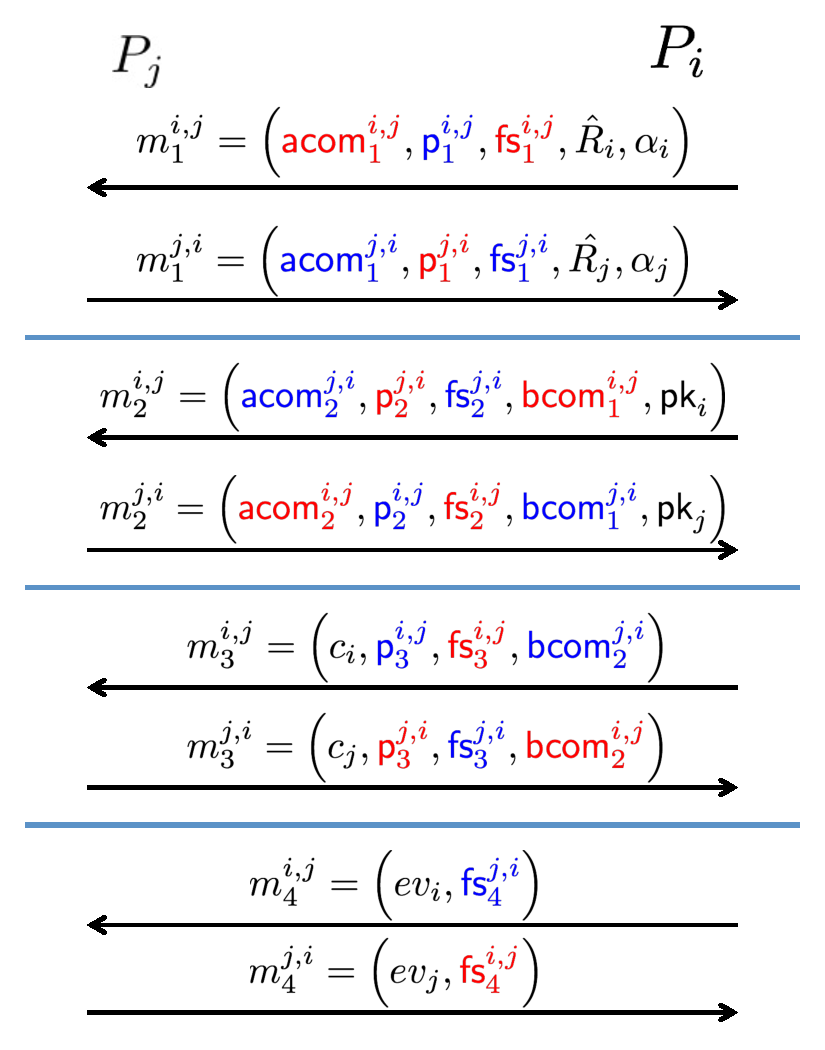
\includegraphics[width=2.8in,height=3.2in]{msg.pdf}}}
\caption{Messages exchanged between party $P_i$ and $P_j$ in $\Pi_\PC$.
  $(\nm_1,\nm_2)$ and $(\onm_1,\onm_2)$ are commitments, $(\WIPOKmsg_1, \WIPOKmsg_2, \WIPOKmsg_3)$ belong to the 3-round $\Pi_\WIPOK$, $(\FLSmsg_1, \FLSmsg_2, \FLSmsg_3,\FLSmsg_4)$ belong to the 4-round $\Pi_\FLS$, and $(\alpha,\pk,c,ev)$ denote the $\MFHE$ messages. Blue messages are sub-protocols where party $P_i$ is the prover/committer and party $P_j$ is the verifier/receiver, red messages are the opposite.}
\label{messages}
\vspace{-3ex}
\end{figure}\anti{I have to update the colored picture to include the $f_i$}
%\begin{figure}
\begin{center}
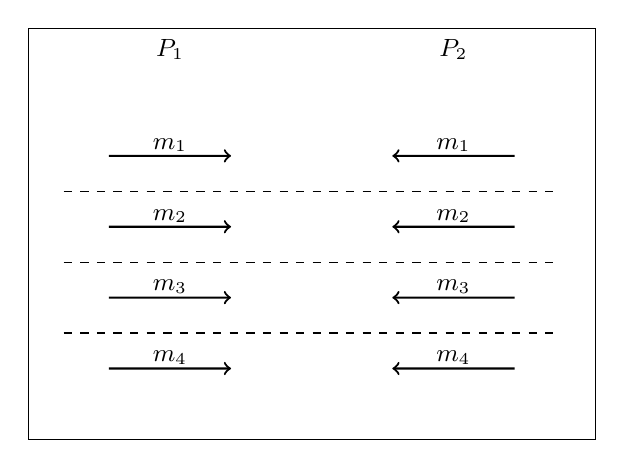
\begin{tikzpicture}
[
	xscale	= 1.8,	% to scale horizontally everything but the text
	yscale	= 1.8,	% to scale vertically everything but the text
]
\node (MS1121) [draw = none] at	(-1.5,-3.5) {};
\node (ME1121) [draw = none] at	(-0.5,-3.5) {};
\node (MS1122) [draw = none] at	(-1.5,-4.0) {};
\node (ME1122) [draw = none] at	(-0.5,-4.0) {};
\node (MS1123) [draw = none] at	(-1.5,-4.5) {};
\node (ME1123) [draw = none] at	(-0.5,-4.5) {};
\node (MS1124) [draw = none] at	(-1.5,-5.0) {};
\node (ME1124) [draw = none] at	(-0.5,-5.0) {};

\node (MS1211) [draw = none] at	(1.5,-3.5) {};
\node (ME1211) [draw = none] at	(0.5,-3.5) {};
\node (MS1212) [draw = none] at	(1.5,-4.0) {};
\node (ME1212) [draw = none] at	(0.5,-4.0) {};
\node (MS1213) [draw = none] at	(1.5,-4.5) {};
\node (ME1213) [draw = none] at	(0.5,-4.5) {};
\node (MS1214) [draw = none] at	(1.5,-5.0) {};
\node (ME1214) [draw = none] at	(0.5,-5.0) {};
%\node (K0) [draw = none] at	(-7.5,-5.5) {};
%\node (K1) [draw = none] at	(-6.5,-5.5) {};


\draw (-2,-5.5) -- (2,-5.5) -- (2,-2.6) -- (-2,-2.6) -- (-2,-5.5);
%\draw (-9,-7) -- (-2,-7) -- (-2,-2) -- (-9,-2) -- (-9,-7);

\node (P11) [draw = none] at	(-1,-2.75) {\small $P_1$};

\node (P12) [draw = none] at	(1,-2.75) {\small $P_2$};


%%%%%%%%%%%mmmmm%%%%%%%%%%%%%%%%%%%%

\node (m11) [draw = none] at	(-1,-3.425) {\small $m_1$};

\node (m12) [draw = none] at	(-1,-3.925) {\small $\tld{m}_2$};

\node (m13) [draw = none] at	(-1,-4.425) {\small $m_3$};

\node (m14) [draw = none] at	(-1,-4.925) {\small $\tld{m}_4$};

\node (m21) [draw = none] at	(1,-3.425) {\small $\tld{m}_1$};

\node (m22) [draw = none] at	(1,-3.925) {\small $m_2$};

\node (m23) [draw = none] at	(1,-4.425) {\small $\tld{m}_3$};

\node (m24) [draw = none] at	(1,-4.925) {\small $m_4$};
\draw
[
thick,
->
]
(MS1121) to (ME1121);
\draw
[
thick,
->
]
(MS1122) to (ME1122);
\draw
[
thick,
->
]
(MS1123) to (ME1123);
\draw
[
thick,
->
]
(MS1124) to (ME1124);

%%%%OTHER DIRECTION CASE-1%%%%%
\draw
[
thick,
->
]
(MS1211) to (ME1211);
\draw
[
thick,
->
]
(MS1212) to (ME1212);
\draw
[
thick,
->
]
(MS1213) to (ME1213);
\draw
[
thick,
->
]
(MS1214) to (ME1214);

%\node (empty) [draw=none] at (-3.5,-3.25) {$\stackrel{\footnotesize Rescheduled}{\large{\implies}}$};

%%%%%%%%%%%%%%Rounds%%%%%%%%%%%%%

\draw
[
dashed,
]
(-1.75,-3.75) to (1.75,-3.75);

\draw
[
dashed,
]
(-1.75,-4.25) to (1.75,-4.25);

\draw
[
dashed,
]
(-1.75,-4.75) to (1.75,-4.75);




\end{tikzpicture}
\end{center}
\caption{2-PC in the simultaneous message exchange model.}
\label{fig:2-PC}
\end{figure}

%%%%%%%%%%%%%%%%%%%%%%%%%%%%%%












% !TEX root =../main-optimal.tex
%%%%%%%%%%%%%%%%%%%%%%%%%%%%%%%%%%%%%%%%%%%%%%%%%%%%%%%%%%%%%%%%%%%%%%
\subsection{Proof of Security} \label{sec:secProof}
%%%%%%%%%%%%%%%%%%%%%%%%%%%%%%%%%%%%%%%%%%%%%%%%%%%%%%%%%%%%%%%%%%%%%%
\BT 
%Let $\ell_{in}, \ell_{out} \in \NN$ and let $F : (\bit^{\ell_{in}})^N \rightarrow \bit^{\ell_{out}}$ be any deterministic polynomial-time $N$-party functionality. 
Assuming sub-exponential hardness of $\LWE$, and the existence of an adaptively-secure commitment scheme, there exists a four-broadcast-round protocol for securely realizing any functionality against malicious adversary in the plain model with no setup.
\label{thm:main}
\ET

To prove \thmref{main}, we note that the two assumptions listed suffice for instantiating all the components of our protocol $\Pi_{\PC}$: The commitment is used directly for $\nmCom$ and $\Com$, and sub-exponential LWE suffices for everything else.
%\anti{make the theorem nicer}
%
Below we prove security of $\Pi_{\PC}$ by describing a simulator and proving that the simulated view is indistinguishable from the real one.

\subsubsection{Description of the Simulator}\label{sec:simu}

Let $\cA$ be a malicious, static adversary that interacts with parties running the protocol $\Pi_\PC$ from Figure \ref{MPC} in the plain model. We construct a simulator $\cS$ (the ideal world adversary) with access to the ideal functionality $\mathbf{\func}$, which simulates a real execution of $\Pi_\PC$ with $\cA$ such that the ideal world experiment with $\cS$ and $\mathbf{\func}$ is indistinguishable from a real execution of $\Pi_\PC$ with $\cA$. Our simulator $\cS$ proceeds as follows:



\paragraph{Simulating actual protocol messages in $\Pi$:} Let $\ccP = \{P_1,\ldots, P_N\}$ be the set of parties participating in the execution of $\Pi_\PC$. Also let $\ccP^* \subseteq \ccP$ be the set of parties corrupted by the adversary $\cA$. The simulator $\cS$ only generates messages on behalf of parties $\ccP\backslash \ccP^*$. %Without loss of generality we assume that only one party is honest, denoted by $P_h$.


\paragraph{Round 1 Messages $\cS \rightarrow \cA$:} In the first round $\cS$ generates messages on behalf of each honest party $P_h \notin \ccP^*$, as follows:

\BE
\item Choose randomness $r_h=(r^{gen}_h,r^{enc}_h)$ for the $\MFHE$ protocol and an unrelated $\kappa$-bit randomness value~$R_h$, and set $\hat{R}_h=OWF(R_h)$.

\item For every $j$ engage in a two-round commitment protocol with $P_j$. To this end, prepare the first message $\nm_1^{h,j}$ corresponding to the execution of $\nmCom_{\id_j}(x_j,r^{gen}_j,r^{enc}_j,R_j;\omega_{j})$ on behalf of $P_h$, acting as the receiver of the commitment.  Since the commitment $\nmCom$ is a two-round protocol, the message of the committer $P_j$ is only sent in the second round. 

\item Prepare the first message $\WIPOKmsg^{h,j}_1$ of $\Pi_\WIPOK$, where $P_h$ acts as the Prover, for the $\NP$-Language $\hhstPOK$ and the first message $\FLSmsg^{h,j}_1$ of $\Pi_\FLS$ where $P_h$ acts as the Verifier for $\stFLSS$. 

\item Honestly generate the message $\alpha_h$ of the $1$-round protocol $\sf \Pi_{GenSetup}$.

\item It then sends the message $m^{h,j}_1=\left(\hat{R}_h, \nm_1^{h,j}, \WIPOKmsg_1^{h,j},\FLSmsg_1^{h,j},\alpha_h\right)$
 to $\cA$.
\EE

     
     

\paragraph{Round 1 Messages $\cA \rightarrow \cS$:} Also in the first round the adversary $\cA$ generates the messages $m^{j,h}_1=\left(\hat{R}_j, \nm_1^{j,h}, \WIPOKmsg_1^{j,h},\FLSmsg_1^{j,h},\alpha_j\right)$ on behalf of corrupted parties $j\in\ccP^*$ to honest parties $h\notin\ccP^*$. Messages $\{\nm_1^{j,h}\}$ correspond to an execution of $\nmCom_{\id_h}({\bf 0};\omega_{h})$.



\paragraph{Round 2 Messages $\cS \rightarrow \cA$:}  In the second round $\cS$ generates messages on behalf of each honest party $P_h\in \ccP^*$ as follows:

\BE 
\item Complete the commitment to the zero string generating the second messages $\nm_2^{j,h}$ corresponding to all executions of $\nmCom_{\id_h}({\bf 0};\omega_{h})$.

\item Honestly prepare the second message $\WIPOKmsg_2^{j,h}$ ($\FLSmsg_2^{j,h}$) of $\Pi_\WIPOK$($\Pi_\FLS$) initiated by $P_j$ acting as the prover (verifier) in the first round. 

\item Generate the second commitment messages $\onm_1^{h,j}$ for $\Com_{\id_j}({\bf 0};\zeta_j)$ where party $P_h$ acts as the Receiver.

\item Generate the individual key pair by locally computing the matrix~$A$ (on input $\{\alpha_i\}_{i\in[N]}$), and by  computing $(\pk_h, \sk_h) = \Keygen(\params, A;r^{gen}_h)$.

\item It then sends the message $m^{h,j}_2:=(\nm^{j,h}_2, \onm^{h,j}_1, \WIPOKmsg^{j,h}_2, \FLSmsg^{j,h}_2,\pk_h)$ to $\cA$.
\EE


\paragraph{Round 2 Messages $\cA \rightarrow \cS$:} In the second round the adversary $\cA$ generates the messages $m^{j,h}_2:=(\nm^{h,j}_2, \onm^{j,h}_1, \WIPOKmsg^{h,j}_2, \FLSmsg^{h,j}_2,\pk_j)$ on behalf of corrupted parties $j\in\ccP^*$ to honest parties $h\notin\ccP^*$. Messages $\{\nm^{h,j}_2\}$ correspond to an execution of $\nmCom_{\id_j}(x_j,r^{gen}_j,r^{enc}_j,R_j;\omega_{j})$ and messages $\{\onm^{j,h}_1\}$ correspond to an execution of $\Com_{\id_h}({\bf 0};\zeta_{h})$


\paragraph{Round 3 Messages $\cS \rightarrow \cA$:}  In the third round $\cS$ generates messages on behalf of each honest party $P_h\notin\ccP^*$ as follows:

\BE
\item Generate the second messages $\onm_2^{j,h}$ corresponding to all $\Com_{\id_h}({\bf 0};\zeta_h)$. 

\item Generate an encryption of the zero string using randomness $r^{enc}_h$, i.e.  $c_h=\Encrypt(pk_h,{\bf 0};r^{enc}_h)$.

\item Honestly prepare the final message $\WIPOKmsg_3^{h,j}$ ($\FLSmsg_3^{h,j}$) of $\Pi_\WIPOK$($\Pi_\FLS$) initiated by $P_h$ acting as the prover (verifier) in the first round. 

\item It sends the message $m^{h,j}_3=(\onm^{j,h}_2,c_h, \WIPOKmsg^{h,j}_3,\FLSmsg^{h,j}_3)$ to $\cA$.
\EE

\paragraph{Round 3 Messages $\cA \rightarrow \cS$:} In the third round $\cA$ generates $m^{j,h}_3=(\onm^{h,j}_2,c_j, \WIPOKmsg^{j,h}_3,\FLSmsg^{j,h}_3)$ where messages $\{\onm^{h,j}_2\}$ correspond to an execution of $\Com_{\id_j}({\bf 0};\zeta_{j})$.
Then, $\cS$ proceeds to extract the witness corresponding to each proof-of-knowledge completed in the first three rounds (via rewinding). To this end, $\cS$ applies the knowledge extractor of $\Pi_\WIPOK$ to obtain the ``witnesses'' which consist of the inputs and secret keys of the corrupted parties $(x_{j},r_j)$\footnote{For simplicity of exposition, we omit the rest of the witness values.} and the zero knowledge simulator of $\Pi_\FLS$ to obtain the ``trapdoors'' (which for a Feige-Shamir protocol means extracting the verifier-secret). If extraction fails, $\cS$ outputs $\mathsf{fail}$. Next $\cS$ sends $\{x_j\}_{j\in[N]\setminus{\{h\}}}$ to the ideal functionality $\mathbf{\func}$ which responds by sending back $y$ such that $y = F(\{x_j\}_{j \in [N]})$.


\paragraph{Round 4 Messages $\cS \rightarrow \cA$:}  In the fourth round $\cS$ generates messages on behalf of each honest party $P_h\notin\ccP^*$ as follows:
\BE
\item Generate the evaluated ciphertext $\hc:= \Evall(\params; F; (c_1,\ldots, c_N))$.
\item Then, $\cS$ obtains all the secret keys $\{\sk_j\}_{j\in\ccP^*}$ reconstructed from the wintesses $\{r^{gen}_j\}_{j\in\ccP^*}$ and computes the simulated decryption shares $\{ev_h\}_{h\notin\ccP^*}\leftarrow \cS^T(y, \hc,h,\{\sk_j\}{_{j\in\ccP^*}})$. (The simulator $\cS^T$ is the one provided by \cite[Section~6.2]{MW16}.)
\item Fake the final message $\FLSmsg^{j,h}_4$ of $\Pi_\FLS$ protocol using the extracted trapdoor.
It sends the message $m^{h,j}_4=(ev_h, \FLSmsg^{j,h}_4)$ on behalf of $P_h$. 
\EE



\paragraph{Round 4 Messages $\cA \rightarrow \cS$:} In the last round the adversary $\cA$ generates the messages on behalf of corrupted parties in $\ccP^*$. For each party $j\in\ccP^*$ our simulator receives messages ${m}^{j,h}_4=({ev}_j, \tFLSmsg^{h,j}_4)$ from $\cA$.

This completes the description of the simulator.







%%%%%%%%%%%%%%%%%%%%%%%%%%%%%%%%%%%%%%%%%%%%%%%%%%%%%%%%%%%%%%%%%%%%%%%%%%%%
\subsubsection{Proof of Indistinguishability}
We need to prove that for any malicious (static) adversary $\cA$, the view generated by the simulator $\cS$ above is indistinguishable from the real view, namely:
$$
\left\{\ideall_{\mathbf{\func},\cS}(\kappa,\cdot)\right\}_{\kappa} \indist
\left\{\reall_{\Pi,\cA}(\kappa,\cdot)\right\}_{\kappa}
$$
To prove indistinguishability, we consider a sequence of hybrid experiments $H_0,H_1,\ldots$ as described below. Let $H_0$ be the hybrid describing the real-world execution of the protocol. We modify this game in steps as follows:

\begin{itemize}
\item[$H_1$] Use the zero-knowledge simulator to generate the proof in the $4$-round $\Pi_{\FLS}$, indistinguishability follows by the ZK property of $\Pi_{\FLS}$.
\item[$H_2$] Starting in this hybrid, the challenger is given access to a breaking oracle $\calB_{\tagg}$ (with $\tagg=(\id_h,\star)$ where $h$ is a honest party). Here the challenger uses the breaking oracle to extract the values committed to by the adversary in $\nm_2^{h,\cA}$ (in the second round), then commits to these same values in $\onm_2^{\cA,h}$ on behalf of the honest party (in the third round). Indistinguishability follows by the adaptive-hiding of $\Com$.

\item[$H_3$] Change the proof in $\Pi_{\WIPOK}$ to use the ``OR branch''. Indistinguishability follows by the WI property of $\Pi_{\WIPOK}$ (which must hold even in the presence of the breaking-oracle $\calB_{\tagg}$). 

\item[$H_4$] Here the challenger also has access to the ideal-world functionality that gives it the output of the function. Having extracted the secret keys using $\calB_{\tagg}$, the challenger \emph{simulates the decryption shares} of the honest parties rather than using the decryption procedure.
  Indistinguishability follows since the FHE scheme is simulatable (which follows from $\LWE$).

\item[$H_5$] Encrypt $0$'s rather than the true inputs. Indistinguishability follows due to the semantic security of the encryption scheme (that follows from the ILWE-hardness of our scheme, under LWE).

\item[$H_6$] Commit to $0$'s in $\nm_2^{\cA,h}$, rather than to the real inputs. Indistinguishable due to the adaptive-hiding of $\nmCom$.

\item[$H_7$] Revert the change in $H_3$, make the proof in $\Pi_{\WIPOK}$ use the normal branch rather than the ``OR branch''. Indistinguishability follows by the WI property of $\Pi_{\WIPOK}$.

\item[$H_8$] Revert the change in $H_2$ and thus commit to zero in $\onm_2^{\cA,h}$ (instead of committing to the extracted values).  Indistinguishability follows by the adaptive-hiding of $\Com$.

\item[$H_9$] Here the challenger no longer has access to a breaking oracle, and instead it uses the POK extractor to get the randomness and inputs (witnesses) from $\Pi_{\WIPOK}$. Indistinguishability follows from the extraction property of $\Pi_{\WIPOK}$, combined with the one-wayness of $OWF$.
\end{itemize}
As $H_9$ we no longer uses the inputs of the honest parties, the view of this hybrid can be simulated. (We also note that the simulator \emph{does not use a breaking oracle}, rather it is a traditional rewinding simulator.)


\paragraph{Security in the presence of a breaking oracle:}
Note that some of our indistinguishability arguments must holds in worlds with a breaking oracle $\calB_{\tagg}$. In particular, we require that $\Com$ is still hiding, that LWE still holds, and that $\Pi_{\WIPOK}$ is still witness-indistinguishable in the presence of the oracle. The hiding property of $\Com$ follows directly from its adaptive-hiding property. As for LWE and $\Pi_{\WIPOK}$, security in the presence of $\calB_{\tagg}$ follows from sub-exponential hardness and complexity leveraging. Namely, in the relevant reductions we can implement $\calB_{\tagg}$ ourselves in subexponential time, while still relying on the hardness of LWE or $\Pi_{\WIPOK}$.

Another point to note is that using the zero-knowledge simulator (in hybrids $H_2$-$H_9$) requires rewinding, which may be problematic when doing other reductions. As we explain below, we are able to handle rewinding by introducing many sub-hybrids, essentially cutting the distinguishing advantage by a factor equals to the number of rewinding operations.


\BDE
\item{$\bf H_0$:} This hybrid is the real execution. In particular, $H_0$ starts the execution of $\cA$ providing it fresh randomness and input $\{x_j\}_{P_j \in\ccP^* }$, and interacts with it honestly by performing all actions of the honest parties with uniform randomness and input. The output consists of $\cA$'s view.


\smallskip
\item{$\bf H_1$:} In this hybrid the challenger uses the zero-knowledge simulator of $\Pi_{\FLS}$ to generate the proofs on behalf of each honest party~$\P_h$, rather than the honest prover strategy as is done in ${\bf H_0}$.
  We note that the challenger in this hybrid needs to rewind the adversary $\cA$ (up to the second round) as needed for the Feige-Shamir ZK simulator.

  Since in these two hybrids the protocol $\Pi_{\FLS}$ is used to prove the same true statement, then the simulated proofs are indistinguishable from the real ones, so we get:
  
\BL $\Hyb{0} \statind  \Hyb{1}$.\EL


\smallskip
\item{$\bf H_2$:} In this ``mental-experiment hybrid'' the challenger is given access to a breaking oracle $\calB_{\id_h}$, with the tag being the identity of an arbitrary honest parties ($h\notin\ccP^*$).
  The challenger begins as in the real execution for the first two rounds, but then it uses $\calB_{\tagg}$ to extract the values $(x_j,r_j,R_j)$ of all the adversarial players $j\in\ccP^*$ from $\nm_2^{h,j}$.

  Then the challenger changes the commitments $\onm_2^{j,h}$ on behalf of the honest party $P_h$, committing to the values $R_j$ that were extracted from $\nm_2^{h,j}$ (and thus making the language $\hhtwost$~--the ``OR branch''--~in $\Pi_{\WIPOK}$ a true statement).%
\footnote{The commitment $Com$ starts in the second round, but this is a two-round commitment so the committed value only affects the second message in the commitment, which happens in the third round of the larger protocol.}

\BL\label{lemmab}$\Hyb{1} \compind  \Hyb{2}$.\EL
\begin{proof}
Since the only differences between these hybrids are the values committed to in $\onm^{j,h}$, then indistinguishability should follow from the adaptive-hiding of the commitment scheme $\Com$ (as the challenger never queries its breaking oracle with any tag containing the identity $\id_h$ of the honest party).

One subtle point here, is that in both $\Hyb{1}$ and $\Hyb{2}$ we use the rewinding Feige-Shamir ZK simulator, so we need to explain how the single value $\onm_2^{j,h}$ provided by the committer in the reduction (which is a commitment to either $0$ or $R_j$) is used in all these transcripts. To that end let $M$ be some polynomial upper bound on the number of rewinding operations needed by the zero-knowledge simulator. The reduction to the security of~$\Com$ will choose at random $t\in[1,M]$ and will only use the $\Com$ committer that it interacts with to commit to a value in the $t$'th rewinding, committing to $0$ in all the rewindings $i<t$ and to the value $R_j$ (that it has from the breaking oracle) in all the rewindings $i>t$.

By a standard argument, if we can distinguish between $\Hyb{1} \compind  \Hyb{2}$ with probability $\epsilon$ then the reduction algorithm can distinguish commitments to 0 and $R_j$ with probability $\epsilon/M$.
\end{proof}

\smallskip
\item{$\bf H_3$:} In this hybrid, we change the witness used in $\Pi_\WIPOK$ on behalf of each honest party $P_h$. In particular, all $\Pi_\WIPOK$ executions use the ``OR branch'' $\hhtwost$.

\BL\label{wipok}$\Hyb{2} \compind  \Hyb{3}$.\EL

\begin{proof}
We make sub-hybrids that change one honest party at a time, and show that a distinguisher $D$ that distinguishes two such sub-hybrids can be used by another distinguisher $D'$ to distinguish between the two witnesses of $\Pi_{WIPOK}$ (as per \defref{dWI}).

%%%%%%%%%%%%%%%%%%%%%%%%%%%%%%%%%%%%%
{\bf Description of $D'$}: $D'$ plays the role of both the challenger and the adversary in the two hybrids, except that the prover messages of $\Pi_\WIPOK$ (on behalf of $P_h$) are obtained from the external prover that the WI-distinguisher $D'$ has access to.

At the third round of the protocol, $D'$ has the statement that $P_h$ needs to prove, and it gets the two witnesses for that statement from the witness-selecting machine in \defref{dWI}. Sending the statement and witnesses to its external prover, $D'$ obtains the relevant $\Pi_\WIPOK$ message (for one of them). $D'$ also uses these witnesses to complete the other flows of the protocol (e.g., the commitments $\onm_2^{j,h}$ that include some of these witnesses). Once the protocol run is finished, it gives the transcript to $D$ and outputs whatever $D$ outputs.

As above, we still need to support rewinding by the Feige-Shamir ZK simulator, while having access to only a single interaction with the external prover, and we do it by sub-sub-hybrids where we embed this interaction in a random rewinding~$t$, producing all the other proofs by the $H_2$ challenger (for $i<t$) or the $H_3$ challenger (for $i>t$). It is clear that the advantage of $D'$ is a $1/M$ fraction of the advantage of~$D$.
\end{proof}

\medskip
We note that $D'$ above still uses the breaking oracle $\calB_{\tagg}$ (to extract the $\Pi_{\FLS}$ secrets), so we need to assume that delayed-input-WI holds even in a world with the breaking oracle. As explained above, we rely on complexity leveraging for that purpose. That is, we let $D'$ run in subexponential time (so it can implement $\calB_{\tagg}$ itself), and set the parameters of $\Pi_\WIPOK$ large enough so we can assume witness-indistinguishability even for such a strong~$D'$. (We can implement subexponential WI protocol from subexponential LWE.)

\smallskip
%%%%%%
\item{$\bf H_4$:} The difference from $H_3$ is that in $H_4$ we simulate the decryption shares of the honest parties. More specifically, the challenger in $H_4$ has access also to the ideal functionality, and it proceeds as follows:
\BE
\item It completes the first three broadcast rounds exactly as in $H_3$.

\item Having extracted the input of all the corrupted parties, the challenger sends all these inputs to the ideal functionality $\mathbf{\func}$ and receives back the output $y = F(\{x_j\}_{j \in [N]})$.

\item Having extracted also all the secret keys of the corrupted parties, the challenger has everything that it needs to compute the simulated decryption shares of the honest parties, $\{ev_h\}_{h\notin\ccP^*}\leftarrow \cS^T(y, \hc,h,\{\sk_j\}{_{j\in\ccP^*}})$.

\item The challenger computes also the last message of $\Pi_{\FLS}$ (using the simulator as before), and sends it together with decryption shares $\{ev_h\}_h$ in the last round.
\EE

%%%%%
\BL$\Hyb{3} \statind  \Hyb{4}$.\EL
\begin{proof}
  The only change between these two experiments is that the partial decryption shares of the honest parties are not generated by partial decryption. Instead they are generated via the the threshold simulator $\cS^T$ of the $\MFHE$ scheme. By the simulatability of threshold decryption, the partial decryptions shares are statistically indistinguishable.
\end{proof}


\smallskip
\item{$\bf H_5$:} 
We change $H_4$ by making $\cS$ broadcast encryptions of ${\bf 0}$ on behalf of the honest parties in the third round, instead of encrypting the real inputs. 
\smallskip
\BL$\Hyb{4} \compind  \Hyb{5}$.
\label{lem:Hyb5-6}
\EL
\begin{proof}
The proof follows directly from semantic security, which in our case follows from LWE. As in the previous hybrid, here too we need this assumption to hold even in the presence of a breaking oracle, and we lose a factor of $M$ in the distinguishing probability due to rewinding.
\end{proof}

\smallskip
\item{$\bf H_6$:} In this hybrid, we get rid of the honest partys' inputs $\{(x_h,r_h)\}_h$ (that are present in the values of $\nm_2^{j,h}$). Formally, $H_6$ is identical to $H_5$ except that in the first round it sets $x_h={\bf 0}$ for all $h\notin\ccP^*$.

\BL$\Hyb{5} \compind  \Hyb{6}$.\EL

\begin{proof}
  This proof is very similar to the the proof of $\Hyb{1} \compind  \Hyb{2}$, and indistinguishability follows from adaptive-hiding of $\nmCom$. Since the challenger never asks its breaking oracle $\calB_{\tagg}$ to break commitments relative to the honest party's tags (and since these committed values are no longer used by the challenger for anything else), then having the honest parties commit to $x_h$ is indistinguishable from having it commit to ${\bf 0}$.
\end{proof}

\smallskip
\item{$\bf H_7$:} In this hybrid we essentially reverse the change that was made in going from $H_2$ to $H_3$. Namely, since now both the encryption and the commitment at each honest party are for the value ${\bf 0}$ then there is no need to use the ``OR branch'' in $\Pi_{\WIPOK}$. Hence we return in using the honest prover strategy there, relative to the input $x_h=0$. As in Lemma \ref{wipok} indistinguishability follows by the WI property of $\Pi_{\WIPOK}$. 

\smallskip
\item{$\bf H_{8}$:} Revert the change that was made in going from $H_1$ to $H_2$ and thus commit to a random value $s_h$ in $\onm_2^{j,h}$.  Indistinguishability follows by the computational hiding of $\Com$, just like in Lemma \ref{lemmab}.

\smallskip
\item{$\bf H_{9}$:} In this hybrid the challenger no longer has access to the breaking oracle $\calB_{\tagg}$. Instead, it uses the knowledge extractor of $\Pi_{\WIPOK}$ to get the input and secret keys of the corrupted parties, and the ``standard'' zero-knowledge simulator to get the proof in $\Pi_{\FLS}$.

\BL$\Hyb{8} \statind  \Hyb{9}$.\EL

\begin{proof}
  The only difference between these hybrids is the method used by the challenger to extract the adversary secrets. Two technical points needs to be addressed here:
  \begin{itemize}
  \item
    This hybrid requires rewinding by \emph{both} the FS ZK simulator and the FLS knowledge extractor, so we need to argue that after polynomially many trials they will \emph{both succeed} on the same transcript. This is a rather standard argument (which essentially boils down to looking at the knowledge-extractor inside $\Pi_{\FLS}$ and the one used explicitly in $\Pi_{\WIPOK}$ as extracting knowledge for and AND language.)

  \item
    We also need to argue that the value extracted from the adversary by the $\Pi_{\WIPOK}$ extractor in $\Hyb{9}$ is a witness for $\onest$ and not for $\twost$. This is done by appealing to the one-wayness of $OWF$, if there is a noticeable probability to extract an $\twost$ witness in $H_9$ then we get an inverter for this one-way function.
  \end{itemize}
  We conclude that in both $\Hyb{8}$ and $\Hyb{9}$ we succeed in extraction with about the same probability, and moreover extract the very same thing, and (statistical) indistinguishability follows.
\end{proof}
\EDE
We conclude the proof by observing that the hybrid $H_9$ is identical to the ideal-world game with the simulator.
\qed

